\chapter{Introduction}


Prediction of molecule properties is an important task in materials design and
drug discovery. This is because when a data set of molecules can be filtered
before starting experimental test, both time and money are saved, leading to
a faster development of novel drugs and materials. However, the use of ab initio
quantum chemical algorithms are currently intractable due to their high
computational cost. Since the chemical space of drugable molecules is estimated
to be $10^{60}$, more efficient algorithms are necessary. One approach is the
use of machine learning (ML) algorithms, as these algorithms are able to find complicated
patterns in large data sets. The problem with ML algorithms is that the best
performing are commonly black boxes, which limits the creation of novel scientific
knowledge. This also results in trust issues in performance critical and highly regulated
environments.


Explainable artificial intelligence (XAI) uses various techniques to explain the prediction
of black box machine learning algorithms. These methods, however, need to take domain knowledge
into account. For example, chemical molecules can be represented as graphs using the Lewis
structure. When existing XAI methods for graph try to explain the most important nodes
or subgraph of a molecule, the result is not very chemically meaningful. This comes from the
fact that chemist do not think in terms of individual atoms, but in substructures such as
functional groups. Recently, Wu et. al. developed substructure graph exploration, where a
molecule is partitioned into different substructures, resulting in a chemical explanation.








\section{Machine learning}

The goal of machine learning is to construct a function $f$, based on parameters
$\pmb{\theta}$, that can accurately predict the outcome variable of the training
data and can generalize to new data.\cite{hastie2009elements} It is common to represent the function input
values (also known as features) as a matrix $\mathbf{X} \in \mathbb{R}^{N \times p}$ where
each row is one sample. Evaluation of the learning function $f$ using the feature matrix
results in the predicted values $\mathbf{\hat{Y}} = f(\mathbf{X}; \pmb{\theta})$. After
obtaining the predicted values, they are compared to the true values (also called labels)
in order to determine how good the model is, which introduces the concept of loss functions $\mathcal{L}$.
Different loss functions exists for different kind of problems.\cite{wang2020comprehensive}
A commonly used loss function is the mean squared error (MSE) (\cref{eq:mse})
which averages the squared difference between the predicted value and true label.
Furthermore, optimizing the loss function with respect to the learning function
parameters produces the best model with the given architecture.\cite{hastie2009elements}


\begin{equation}
	\label{eq:mse}
	\text{MSE}\big(\pmb{y}, \pmb{X}\big) = \frac{1}{N}  \big[\pmb{y} - f(\mathbf{X})\big]^T[\pmb{y} - f(\mathbf{X})\big]
\end{equation}


One of the simplest functions $f\left(\mathbf{X}; \pmb{\theta}\right) = \mathbf{X}\pmb{\theta}$
is a linear combination of the features, where $\pmb{\theta} \in \mathbb{R}^p$
is the vector of coefficients. This model, known as linear regression, is commonly
used in statistical modeling.\cite{kutner2005applied} Although the linear model is
very interpretable, the linearity constraint is too strict which limits its
applicability. Therefore, more complicated ML algorithms were developed which are
able to obtain improved performance on complicated data with respect to linear
regression by allowing non-linear relationships.\cite{deng2012mnist} However,
they pay a price in terms of interpretability.\cite{fan2021interpretability}


\section{Neural networks}


Neural networks are a class of machine learning algorithms which are able to
approximate complicated non-linear function.\cite{cybenko1989approximation} Initially, they where developed as
a simple mathematical model of the human brain.\cite{rosenblatt1962principles} Although this is a strong
simplification, the concept of neuron signal transit is used as a basic building
block for a neural network.\cite{wang2017origin} This signal transmission
takes place between units in a neural network. Then, different architectures
can be used to connect different units. The multi layer perceptron (MLP) is a basic
architecture that is frequently utilized in other, more complicated neural networks.\cite{almeida2020multilayer}
In an MLP (\cref{fig:mlp_structure}) three parts can be distinguished: an input layer,
one or more hidden layers and an output layer.


\begin{figure}[h]
	\centering
	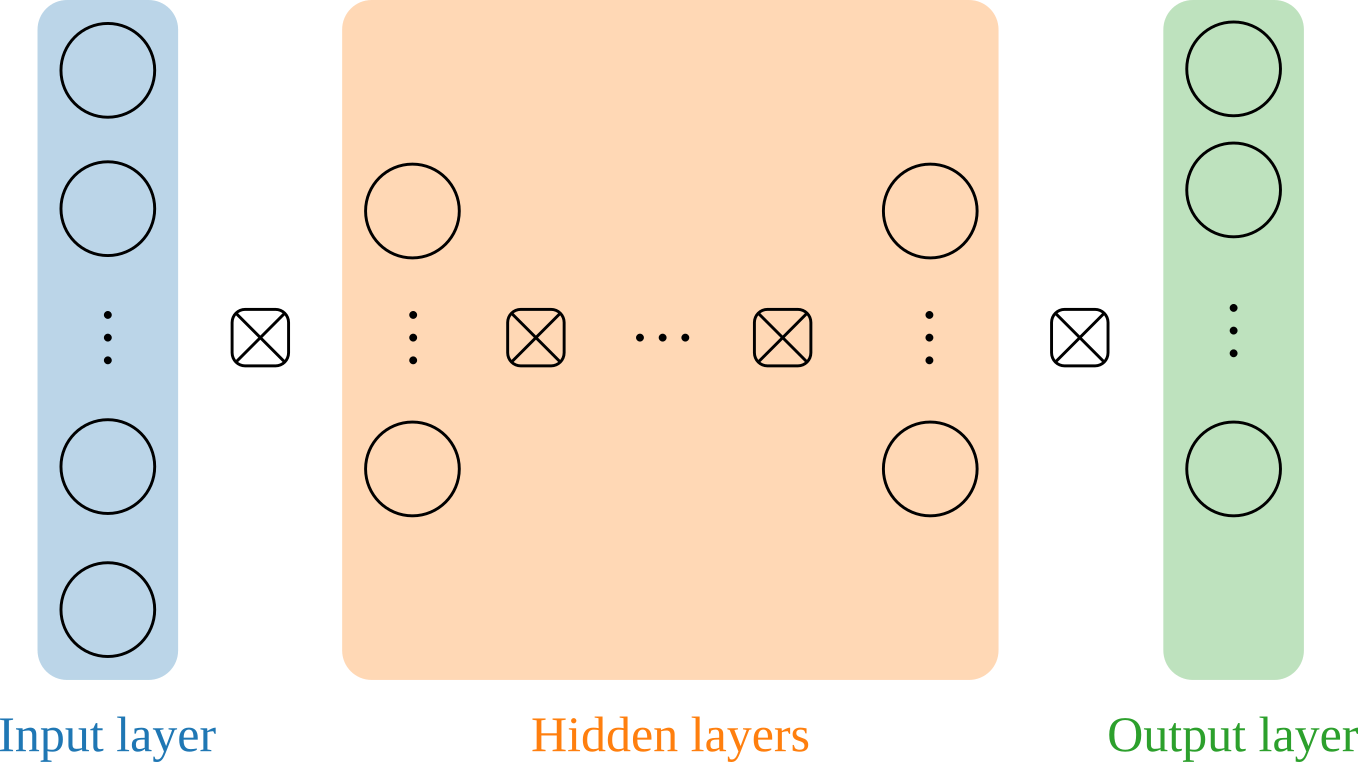
\includegraphics[scale=1.5]{mlp.png}
	\caption{General structure of a multi layer perceptron (MLP) consisting of an input layer,
		one or multiple hidden layers and an output layer. The symbol separating two layers denote that
		all neurons between these two layers are connected.}
	\label{fig:mlp_structure}
\end{figure}


The values of the input layer are equal to the given feature matrix
$\pmb{X}$. Let $n^{(1)}$ denote the number of units in the first hidden layer.
Then taking $n^{(1)}$ different linear combinations of the input layer followed by
a non-linear activation function $\sigma$ results in the values of this first hidden
layer. Generally, the values $\pmb{H}^{(l)} \in \mathbb{R}^{N \times n^{(l)}}$ of layer
$l$ are given by


\begin{equation}
	\pmb{H}^{(l)} =  \sigma^{(l)} \left(\pmb{H}^{(l-1)}\pmb{\Theta}^{(l-1)} \right),
\end{equation}


where $\pmb{\Theta}^{(l-1)} \in \mathbb{R}^{n^{(l-1)} \times n^{(l)}}$ is the weights matrix
of layer $l - 1$, with $n^{(l-1)}$ and $n^{(l)}$ the number of units in layers
$l-1$ and $l$ respectively and $\pmb{H}^{(0)} = \pmb{X}$. Popular activation
functions are listed in \cref{tab:activation_functions}.

\begin{table}[h]
	\caption{Popular activation functions used in multi layer perceptrons.}
	\label{tab:activation_functions}
	\begin{center}
		\begin{tabular}{c|c}
			\toprule
			Sigmoid(x) = $ \frac{1}{1 + e^{-x}}$                 &
			Softmax(x) = $\frac{e^x}{\sum_{i=1}^{n_L} e^{x_i}}$                                                           \\
			\midrule
			ReLU(x)\cite{glorot2011deep} = $\begin{cases}
					                                x & \text{if } x > 0 \\
					                                0 & \text{otherwise}
				                                \end{cases}$        &
			LeakyReLU(x)\cite{maas2013rectifier} =  $\begin{cases}
					                                         x        & \text{if } x > 0 \\
					                                         \alpha x & \text{otherwise}
				                                         \end{cases}$
			\\ & with $\alpha \ge 0$
			\\
			\midrule
			SeLU(x)\cite{klambauer2017self} = $\lambda \begin{cases}
					                                           x               & \text{if } x > 0 \\
					                                           \alpha(e^x - 1) & \text{otherwise}
				                                           \end{cases}$
			                                                     &
			Gelu(x)\cite{hendrycks2016gaussian} = $\begin{cases}
					                                       x            & \text{if } x > 0 \\
					                                       x \, \Phi(x) & \text{otherwise}
				                                       \end{cases}$
			\\
			with $\gamma = 1.05070098$ and $\alpha = 1.67326324$ & with $\Phi(x)$ cumulative standard normal distribution \\
			\bottomrule
		\end{tabular}
	\end{center}
\end{table}

An MLP often does not assess the whole feature matrix at once. Rather, the feature
matrix is split up into many batches. Then, following each batch, the parameters are
updated using an optimization algorithm. Common optimization algorithms in neural networks
are gradient descent and Adam.


\subsection{Gradient descent}


A popular optimization algorithm to optimize the weights $\pmb{\Theta}$ of a neural network is
gradient descent.\cite{ruder2016overview} As the name implies, this algorithm
uses the gradient of the loss function $\mathcal{L}$ to step in the direction of the
steepest decline. The size of this step is determined by the learning rate $\alpha$.

\begin{equation}
	\pmb{\Theta}_{t+1} = \pmb{\Theta}_{t} - \alpha \nabla_{\pmb{\Theta}} \mathcal{L}
\end{equation}

Computation of the gradient can be achieved using the back propagation algorithm, which
propagates the gradient layer by layer through the network starting at the output.
\cite{lecun1988theoretical} A limitation of gradient descent is the fixed learning
rate which must carefully be chosen. One limitation of gradient descent is the
fixed learning rate that has to be chosen thoughtfully at the start of training.
If the learning rate is too large, the step can pass beyond the minimum. Otherwise,
if the learning rate is too small it can take a very long time until convergence.
A possible solution is to stop after a few iterations, adjust learning rate and
continue training. However, this is not really efficient. A better algorithm,
which is nowadays the standard optimization algorithm in deep learning, is Adam.\cite{kingma2014adam}


\subsection{Adam}

Adam uses exponential moving averages to estimate the first $m$ and second $v$
moments of the gradient, where the exponential decay is controlled by the hyperparameters
$\beta_1$ and $\beta_2$. However, these moments have a bias towards zero due to a
zero initialization. Therefore, bias correction is used to obtain unbiased estimates
of the moments $\hat{m}$ and $\hat{v}$.\cite{kingma2014adam}


\begin{subequations}
	\begin{equation}
		m_{t+1} = \beta_1 m_t + (1 - \beta_1) \nabla_{\pmb{\Theta}} f
	\end{equation}
	\begin{equation}
		v_{t+1} = \beta_2 v_t + (1 - \beta_2) \left( \nabla_{\pmb{\Theta}} f \right)^2
	\end{equation}
	\begin{equation}
		\hat{m}_{t+1} = \frac{m_t}{1 - \beta^t_1}
	\end{equation}
	\begin{equation}
		\hat{v}_{t+1} = \frac{v_t}{1 - \beta^t_2}
	\end{equation}
\end{subequations}


Subsequently, the gradients can be updated via


\begin{equation}
	\pmb{\Theta}_{t+1} = \pmb{\Theta}_t - \alpha \frac{\hat{m}_t}{\sqrt{\hat{v}_t} + \epsilon}
\end{equation}


Typical values for the hyperparameters are $\beta_1 = 0.9, \beta_2 = 0.999, \epsilon = 10^{-8}$
and $\alpha = 0.001$.


\section{Graph neural networks}


A graph $\mathcal{G}$ is defined as a pair $\left<\mathcal{V}, \mathcal{E}\right>$
consisting of a set of nodes $\mathcal{V}$ and a set of edges $\mathcal{E}$.
The node feature matrix $\pmb{X}^{(\mathcal{V})} \in \mathbb{R}^{|\mathcal{V}| \times d}$
contains for every node $v \in \mathcal{V}$ a feature vector $\pmb{x}_v \in \mathbb{R}^d$.
Also the edges of a graph can have feature vectors. Let $\{i,j\} \in \mathcal{E}$ be
the edge between nodes $i$ and $j$, then its feature vector is denoted by
$\pmb{e}_{ij} \in \mathbb{R}^c$.\cite{wu2020comprehensive}
Since an MLP can only handle one feature vector per sample as input, it
cannot directly used on graph structured data. A possible solution to this
is the aggregation of the neighbors $\mathcal{N}(i) \coloneqq \{j \in \mathcal{V} | e_{ij} \in \mathcal{E}\}$ of node $i$,
after which the resulting feature vector can be given to an arbitrary vector function
such as an MLP. This is the concept of message passing neural networks (MPNN), which
are generally written as\cite{gilmer2017neural}


\begin{equation}
	\label{eq:mpnn}
	\pmb{h}^{(l + 1)}_i = U\left(\pmb{h}^{(l)}_i, AGG_{j \in \mathcal{N}(i)} M\left(\pmb{h}^{(l)}_i, \pmb{h}^{(l)}_j, \pmb{e}_{ij}\right)\right),
\end{equation}

with $\pmb{h}^{(0)}_i = \pmb{x}_i$, $AGG()$ is an arbitrary aggregation function
for example sum or mean, $M()$ is a message function and $U()$ is the node update function.

Graph neural networks are used to make predictions on three different levels:
nodes, edges and graph. On the node level common tasks are to classify nodes.
For example in a graph where each node represents a financial transaction, predict
whether the transaction was fraudulent or not. Link prediction is an edge level
task that tries to predict to existence of a relation between two nodes. At last
graph level task can perform classification or regression on the whole graph, for
example the prediction of water solubility of small molecules.\cite{wu2020comprehensive}
This requires a representation of the whole graph, which is achieved by a node
aggregation function\cite{gilmer2017neural}

\begin{equation}
	\hat{\pmb{y}} = R(\{\pmb{h}^{(L)}_v | v \in \mathcal{V}\}),
\end{equation}


where $\pmb{h}^{(L)}_v$ is the feature vector of the last MPNN layer.


\subsection{MPNN by Duvenaud et. al.}

Duvenaud et. al. used the message passing framework to generate learned molecule
fingerprints.\cite{duvenaud2015convolutional} In their framework, the message function
$M\left(\pmb{h}^{(l)}_i, \pmb{h}^{(l)}_j, \pmb{e}_{ij}\right) = \pmb{h}_j \mathbin\Vert \pmb{e}_{ij}$
concatenates a neighbor with its corresponding edge. Subsequently the messages are
aggregated by a sum, weighted by a learnable weight matrix $\pmb{\Theta}^{(l, deg(i))}$
one for each layer and node degree. Next, a sigmoid function is applied to provide
the updated node feature vectors. Using the general formula of \cref{eq:mpnn}, this
can be summarized as

\begin{equation}
	\pmb{h}^{(l + 1)}_i = \sigma\left( \pmb{\Theta}^{(l, deg(i))} \sum_{j \in \mathcal{N}(i)}
	\pmb{h}^{(l)}_j \mathbin\Vert \pmb{e}_{ij}\right),
\end{equation}


After $L$ layers the graph prediction is obtained using an MLP and skip connections
to all hidden node feature vectors


\begin{equation}
	\hat{\pmb{y}} = MLP\left(\sum^{|\mathcal{V}|}_i \sum^L_{l=0} softmax\left(\tilde{\pmb{\Theta}}^{(l)} \pmb{h}^{(l)}_i\right)\right)
\end{equation}


A limitation of this architecture is the separate summation over nodes and edges
resulting in the failure to identify correlations between edges and nodes.\cite{wu2020comprehensive}


\subsection{Relational graph neural networks}


Relational graph neural networks (RGCN) use a different approach to combine node
and edge features. Here, edge features are used to give a relation type $\mathcal{R}$
to edges. Then, instead of summing over the whole neighborhood with only one
weight matrix, each relation type $r \in \mathcal{R}$ has its own weight matrix
$\pmb{\Theta}^{(l)}_r$. Then, \cref{eq:mpnn} becomes\cite{schlichtkrull2018modeling}


\begin{equation}
	\pmb{h}^{(l+1)}_i = \sigma \left( \sum_{r \in \mathcal{R}} \sum_{j \in \mathcal{N}(i, r)} \pmb{\Theta}^{(l)}_r \pmb{h}^{(l)}_j
	+ \pmb{\Theta}^{(l)}_0 \pmb{h}^{(l)}_i \right),
\end{equation}


where $\mathcal{N}(i, r)$ are the neighbors of node $i$ with relation type $r$.
A self loop with a weight matrix $\pmb{\Theta}_0$ of special relation
is used preserve information of previous layers.


\section{Explainable machine learning}


\subsection{Shapley value}
\label{subsec:shapley_value}

Feature attribution methods in XAI assign a number to each feature implying how
much that feature contributed to the model prediction.\cite{merrick2020explanation}
In other words, the features cooperate with each other to obtain a payoff given
by the ML model and the interest lies in the contribution of each feature to the
model prediction. These problems are more generally studied in cooperative game
theory. Formally, a cooperative game with transferable utility (i.e. a TU-game) is
defined as a pair $(N, v)$ consisting of a set of players (i.e. the features)
and a characteristic function (i.e. ML model) which satisfies\cite{zhang2022gstarx}


\begin{equation}
	v: 2^N \coloneqq \{S | S \subseteq N\} \rightarrow \mathbb{R}, \quad v\left(\emptyset\right) = 0.
\end{equation}


A solution of a game $\phi(N, v) \in \mathbb{R}^{|N|}$ is a vector where the $i$th element
denotes the contribution of player $i$ to the payoff $v(N)$ obtained by all players
of the coalition $N$.\cite{zhang2022gstarx} Therefore, the solution vector,
also called a value, can be used to provide the attributions of each feature.


A popular value used in machine learning is the Shapley value, which distributes
the total payoff among the players in a mathematical fair manner by satisfying the
following axioms:\cite{merrick2020explanation, shapley1953value}


\begin{itemize}
	\item Dummy player: If a player $i$ does not add to the payoff, then it receives a
	      zero value (i.e. $\forall S \subseteq N: v(S \cup \{i\}) = v(S) \implies \phi_i(N, v) = 0$).

	\item Symmetry: If two players ($i$ and $j$) have the same contribution in all coalitions, then
	      their values are equal (i.e. $\forall S \subseteq N \setminus \{i, j\}: v(S \cup \{i\}) = v(S \cup \{j\}) \implies \phi_i(N, v) = \phi_j(N, v)$).

	\item Efficiency: The sum of the attributions of all players equals the payoff of the coalition containing
	      all players (i.e. $\sum^{|N|}_i \phi_i(N, v) = v(N)$).

	\item Linearity: The value of a game where the characteristic function $v$ is a linear combination of
	      two other value functions $u$ and $w$, then the value is also a linear combination (i.e.
	      $v = \alpha u + \beta w \implies \phi(N, v) = \alpha \phi(N, u) + \beta \phi(N, w)$)
\end{itemize}


The Shapley value $\phi_i$ of player $i$ is given by the expected marginal contribution\cite{zhang2022gstarx}


\begin{equation}
	m(i) = v\left(S \cup \{i\}\right) - v\left(S\right), \; \text{with } S \subseteq N \setminus \{i\}
\end{equation}


over all possible coalitions


\begin{equation}
	\begin{aligned}
		\label{eq:Shapley}
		\phi_i(N, v) & = \frac{1}{|N|} \sum_{k=0}^{|N|-1} \frac{\left(|N| - 1 - k\right)k!}{\left(|N| - 1\right)!} \sum_{S \subseteq N \setminus \{i\}, |S| = k} m(i) \\
		             & = \sum_{k=0}^{|N| - 1} \sum_{S \subseteq N \setminus \{i\}, |S| = k} \frac{\left(|N| - 1 - |S|\right)|S|!}{|N|!} m(i)                          \\
		             & = \sum_{S \subseteq N \setminus \{i\}} \frac{\left(|N| - 1 - |S|\right)|S|!}{|N|!} m(i)
	\end{aligned}
\end{equation}


assuming that every coalition is equally probable. This last assumption can be questioned whether it should
always hold. For instance, define an unanimity game as a game $(N, u_R)$ with characteristic function


\begin{equation}
	u_R = \begin{cases}
		1 \quad \text{if } R \subseteq S \\
		0 \quad \text{otherwise}
	\end{cases}.
\end{equation}


Then the Shapley value for the unanimity game $(\{1, 2, 3\}, u_{\{1,2,3\}})$ is $1/3$ for every player.\cite{hamiache_value_1999}
Now, suppose players one and three cannot communicate with each other and hence cannot form a coalition.
Since the Shapley value does not account for any communication structure, the Shapley values are still
$1/3$ for all players. However, it would be more intuitive if player two had a higher value, as it can
communicate to more players than players one and three. Because it is possible to represent chemical
structures as graphs, it could be interesting to include the graphical structure in the explanation. A
value that does include a communication structure is the Hamiache-Navarro value.\cite{hamiache_value_1999, hamiache_associated_2020}


\subsection{Hamiache-Navarro value}


Before discussing the Hamiache-Navarro value, some notation is defined. Let a game $(N, v)$ with a
communication structure be a triple $(N, v, g)$, where $g \subseteq g_N \coloneqq \{ \{i, j \} | i, j \in N \}$
is a set of adjacent nodes. The graph $\left< N, g \right>$ specifies the
communication structure, where players $i$ and $j$ can only communicate if they are adjacent
(i.e. $\{i, j \} \in g$). A path is a sequence $i = i_1, i_2, \dots , i_k = j$ of nodes from player
$i$ to player $j$ such that $\{i_q, i_{q+1} \} \in g$ for $1 \le q \le k - 1$. If such a path exists
between two players, then they are connected by the graph $\left<N, g\right>$ which is denoted by
$i \underset{\left< N, g \right>}{\rightarrow} j$. This allows to define a partition
$N/g \coloneqq \{\{ i | i \in N \land i \underset{\left<N, g \right>}{\rightarrow} j\} \cup \{j\} | j \in N \}$
of the set of nodes $N$ over the graph $<N, g>$ as the set of all connected nodes.\cite{hamiache_value_1999}

A coalition $S \subseteq N$ can only directly interact with its connected neighbors. Let
$S^* \coloneqq \{ i \in N | \exists j \in S \text{ such that } \{i, j\} \in g \}$ be the set of players
which are adjacent to at least one player in the coalition $S$. The interconnection of the neighbors of
$S$ is of no importance as the coalition $S$ cannot see them. Therefore, the coalition $S$ can value its
own payoff $v^*(S)$ as its payoff $v(S)$ in the original game and a fraction $\tau$ of the net payoff obtained
by cooperating with each of its connected neighbors separately\cite{hamiache2001associated}


\begin{equation}
	\label{eq:associated_game}
	v^*(S) =
	\begin{cases}
		\displaystyle
		v(S) + \tau \sum_{j \in S^* \setminus S} \left[ v(S \cup \{j\}) - v(S) - v(\{j\}) \right] & \text{if } |S/g| = 1 \\
		\displaystyle
		\sum_{R \in S/g} v^*(R)                                                                   & \text{otherwise}
	\end{cases}
	.
\end{equation}

When the coalition $S$ is not connected (i.e. $|S/g| \ne 1$), then its own payoff is the sum of the self
evaluated payoffs of the components $R \in S/g$ of the coalition $S$.
This introduces a series of associated games $(N, v^*, g)$, $(N, v^{**}, g)$, \dots which converges
to the limit game $(N, \tilde{v}, g)$. An associated game is consistent if its solution is the same
as the solution of the original game. When the graph is complete (i.e. all players are connected to
each other), then the solution of the associated game converges to the Shapley value.\cite{hamiache2001associated}


In what follows, the concept of associated games are converted into a matrix approach.
To be consistent, an order of the matrix columns and rows are defined. Therefore a lexicographic order is defined
for coalitions of the same size. Suppose $A$ and $B$ are coalitions of the same size where the elements are ordered
from small to large (i.e. $a_1 < a_2 < \dots < a_k, \quad a_i \in A$). The coalition $A$ comes lexicographic
before coalition $B$ ($A \prec B$) if and only if $a_1 < b_1$ or $\exists \gamma \in \mathbb{N}, 1 \le i < \gamma: a_i = b_i \land a_\gamma < b_\gamma$.
For two arbitrary coalitions $S$ and $T$, $S < T$ if $|S| < |T|$ or $S \prec T$. Using this ordering, the characteristic
function $v$ of the game $(N, v, g)$ can be represented as a vector in $\mathbb{R}^{2^N - 1}$. The associated game
\cref{eq:associated_game} $v^*_\tau = P_g M_c P_g v$ can then be written as a linear transformation of the characteristic vector
, where the square matrix $M_c$ for two arbitrary coalitions $\emptyset \ne S \subseteq N$
and $\emptyset \ne T \subseteq N$ is given by\cite{hamiache_associated_2020,hamiache2010matrix}


\begin{equation}
	M_c[S, T] =
	\begin{cases}
		1 - |N \setminus S| \tau & \text{if } |S| = |T|                         \\
		\tau                     & \text{if } |S| + 1 = |T| \land S \subseteq T \\
		-\tau                    & \text{if } |T| = 1  \land T \not \subseteq S \\
		0                        & \text{otherwise}
	\end{cases}
\end{equation}


and matrix $P_g$ is given by

\begin{equation}
	P_g[S, T] =
	\begin{cases}
		1 & \text{if } T \in S/g \\
		0 & \text{otherwise}     \\
	\end{cases}
	,
\end{equation}


which represents the graphical structure of the game. This allows to write the series of associated
games as $v^*_\tau = P_g M_c P_g v, v^{**}_\tau = P_g M_c P_g v^*_\tau, \dots, v^{(k*)}_\tau = \left(P_g M_c P_g\right)^k v$.
Provided that $\tau$ is small enough ($\tau < \frac{2}{|N|}$ for complete graphs\cite{hamiache2001associated}),
the power series $\left(P_g M_c P_g\right)^k v$ converges as $k$ tends to infinity.\footnote{A proof can be found in \cite{hamiache_associated_2020}}
The convergence produces a limit game $(N, \tilde{v}, g)$, where the solution $\phi_i$ of player $i$ equals the
payoff $\tilde{v}(\{i\})$ of player $i$.\cite{zhang2022gstarx, hamiache_associated_2020}


\textbf{Numerical example}

In order to compare the Hamiache-Navarro value and the Shapley value the same example as in \cref{subsec:shapley_value}
is used. To recap, define an unanimity game with communication structure $(\{1, 2, 3\}, u_{\{1, 2, 3\}}, \{\{1, 2\}, \{2, 3\}\})$
where $u_{\{1, 2, 3\}}(S)$ is one if $\{1, 2, 3\} \in S$ and zero otherwise with $S \subseteq \{1, 2, 3\}$. As discussed
in \cref{subsec:shapley_value}, the Shapley value is equal to $1/3$ for all players. However, the HN-value is not equal
for all players. Players one and three have an HN-value of $1/4$ and the HN-value for player two is $1/2$
(see \cref{app:HN_example}).\cite{hamiache_associated_2020}
